\documentclass{standalone}
\usepackage{tikz}
\usepackage{ctex,siunitx}
\setCJKmainfont{Noto Serif CJK SC}
\usepackage{tkz-euclide}
\usepackage{amsmath}
\usetikzlibrary{patterns, calc,3d}
\usetikzlibrary {decorations.pathmorphing,decorations.pathreplacing,decorations.shapes}
\tikzset{label style/.append style={font=\small}}
\begin{document}
\small
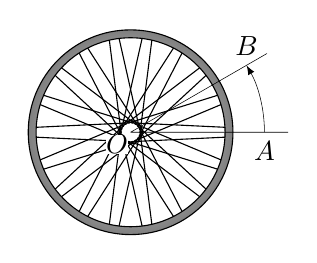
\begin{tikzpicture}[>=latex,scale=1.0]
  \draw[inner color=white,outer color=gray,even odd rule](0,0)circle(1.3)(0,0)circle(1.2);
  \draw(0,0)circle(0.15);
  \foreach \x in {0,20,...,340}
  {
    \draw(\x+3:1.2)--(\x+85:0.12);
    \draw(\x-3:1.2)--(\x-85:0.12);
  }
  \draw[very thin](0,0)--(2,0)(0,0)--(30:2);
  \draw[very thin,->](1.7,0)node[below]{$A$}arc(0:30:1.7)node[above]{$B$};
  \node at (0,0)[below left=1pt,inner sep=0pt,fill=white]{$O$};
\end{tikzpicture}
\end{document}